\documentclass{article}
\usepackage[T1]{fontenc}
\usepackage{lmodern}
\usepackage{graphicx}
\usepackage{amsmath,amssymb}
\usepackage[a4paper,margin=2cm]{geometry}
\usepackage[absolute,overlay]{textpos}
\setlength{\TPHorizModule}{1mm}
\setlength{\TPVertModule}{1mm}
\usepackage[indonesian]{babel}
\usepackage{hyperref}
\setlength{\emergencystretch}{2em}
% unit: Halaman 31

\begin{document}

% === Halaman 31 (llm) ===

\section*{Blaise de Vigen\`ere}

\textbf{Blaise de Vigen\`ere} (French: [\text{vi\textsubscript{z}\textepsilon\textsubscript{r} \textepsilon}]; 5 April 1523 -- 19 February 1596)$^{[1]}$ was a French diplomat, cryptographer, translator and alchemist.

\vspace{205.23mm}

\subsection*{Biography [ edit ]}

Vigen\`ere was born into a respectable family in the village of Saint-Pour\c{c}ain in Bourbonnais. When he was 12, his father, Jehan (modern spelling Jean) de Vigen\`ere, arranged for him to have a classical education in Paris. Registered at the university at 14, he quit after three years without a known degree.$^{[2]}$

\vspace{10mm}

From 1539 to around 1545, he worked under Gilbert Bayard, a first secretary to King Francis I, who had fiefs in Bourbonnais.$^{[2]}$

In 1545, he accompanied the French envoy Louis Adh{\'e}mar de Monteil, Count of Grignan, to the Diet of Worms as a junior secretary.$^{[3][4]}$ After the diet's rupture, he traveled in Europe.$^{[5]}$

In 1547, he quit the court and entered the service of the House of Nevers. He would remain associated with it until at least a year before

Sumber: Wikipedia

% deskripsi: Infobox Wikipedia tentang Blaise de Vigenère yang berisi potret wajah dan rincian biografi seperti tanggal lahir, tanggal wafat, pekerjaan, dan hal yang dikenal.
% bbox normalisasi: [0.5660, 0.2220, 0.7840, 0.9130]
\begin{textblock*}{45.78mm}(118.86mm,65.93mm)
\noindent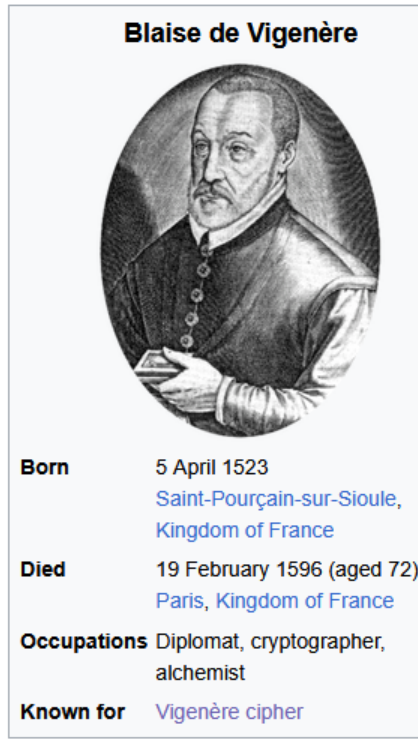
\includegraphics[width=45.78mm,height=205.23mm]{../../images/llm/page_031_img_01.png}%
\end{textblock*}

\end{document}
